\documentclass[final,5p,times]{elsarticle}
\usepackage{graphicx}
\usepackage{subfigure}

\usepackage{amssymb}
\usepackage[nodots]{numcompress}
\usepackage{lineno}
\usepackage[utf8]{inputenc}
\usepackage{caption}
\usepackage{hyphenat}
\usepackage{array}
\usepackage{makecell}

\include{myhyph}

%% Avoids linenumbers to collide with text for 5p format:
\setlength\linenumbersep{3pt}


\journal{Computers \& Graphics}

\begin{document}

\begin{frontmatter}


\title{A novel GPU-based sonar simulator for real-time applications}

% \author[senai,ufba]{Rômulo Cerqueira} \ead{romulo.cerqueira@ufba.br}
% \author[senai]{Tiago Trocoli}
% \author[senai]{Gustavo Neves}
% \author[senai]{Sylvain Joyeux}
% \author[senai,dfki]{Jan Albiez}
% \author[ufba]{Luciano Oliveira}

% \address[senai]{Brazilian Institute of Robotics, SENAI CIMATEC, Salvador, Bahia, Brazil}
% \address[ufba]{Intelligent Vision Research Lab, Federal University of Bahia, Salvador, Bahia, Brazil}
% \address[dfki]{Robotics Innovation Center, DFKI GmbH, Bremen, Germany}

\begin{abstract}

Sonar simulation requires great computational effort due to the complexity of
acoustic physics mainly when applied in the underwater environment. This fact turns the
challenge of reproducing sensor data into a non-trivial task. On the other
hand, simulation of sonar operation data allows to evaluate algorithms and
control systems without going to the real underwater environment; that reduces
the costs and risks of in-field experiments. This paper proposes a novel
real-time underwater imaging sonar simulator, which uses the OpenGL shading
language (GLSL) chain, and is able to simulate two main types of sonar sensors:
mechanical scanning imaging sonars (MSIS) and forward-looking sonars (FLS). The
virtual underwater simulation was conceived based on three frameworks: (i)
OpenSceneGraph (OSG) reproduces the ocean visual effects, (ii) Gazebo deals
with physics effects, and (iii) the Robot Construction Kit (Rock) controls the
sonar in underwater environments. The proposed sonar simulation exploits the
rasterization pipeline in order to build a matrix comprised of echo intensity,
distance and angular distortion, being all calculated over object shapes in
the 3D rendered scene. Sonar-intrinsic speckle noise and object
material properties are also considered as part of the sonar image. Our
evaluation demonstrated that the proposed method is able to operate with high
frame rate, as well as realistic sonar image quality in different virtual
underwater scenarios.

\end{abstract}

\begin{keyword}
Simulated sensor data
\sep sonar imaging
\sep GPU-based processing
\sep Robot Construction Kit (Rock)
\sep Underwater robotics.

\end{keyword}

\end{frontmatter}

%%
%% Start line numbering here if you want
%%
\linenumbers

\section{Introduction}
\label{introduction}

% Importance of simulation for autonomous robots
Simulation is an useful tool for designing and programming autonomous robot
systems. That allows evaluating robot behavior, without dealing with physical
hardware or decision-making algorithms and control systems in real-time
trials, as well as costly and time-consuming field experiments.

When working with autonomous underwater vehicles (AUVs), simulation of
facilities are specially relevant. AUVs usually demand expensive hardware and
perform long-term data gathering operations, taking place in restrictive
sites. As AUV does not need umbilical cable, and the underwater communication
carries on by unreliable acoustic links, the robot should be able to make
completely autonomous decisions, even with low-to-zero external assistance.
While the analysis and interpretation of sensor data can be performed in a
post-processing step, a real-time simulation is strongly needed for testing
and evaluation of vehicle's motion responses, avoiding involved risks on
real world rides.

% Importance of Imaging sonars
AUVs usually act below the photic zone, with high turbidity and huge light
scattering. This makes the quality of image acquisition by optical devices
limited by a short range, and also artificially illuminated and clear visibility
conditions. To tackle with that limitations, high-frequency sonars have been
used primarily on AUVs' navigation and perception systems. Acoustic waves
emitted by sonars are significantly less affected by water attenuation,
aiding operation at greater ranges even as low-to-zero visibility conditions,
with a fast refresh rate. Although sonar devices usually solve the main
shortcomings of optical sensors, they provide noisy data of lower
resolution and more difficult interpretation.

% Related works
By considering sonar benefits and singularities along with the need to
evaluate AUVs, recent works proposed ray tracing- and tube tracing-based
techniques to simulate acoustic data with very accurate results, although
having a high computational cost
\cite{bell1997,coiras2009,gueriot2010,sac2015,demarco2015,gu2013,kwak2015}.
Bell \cite{bell1997} proposed a simulator based on optical ray tracing for
underwater side-scan sonar imagery; images were generated by acoustic
signals represented by rays, which are repeatedly processed, forming a
2D-array. Coiras and Groen \cite{coiras2009} used frequency-domain
signal processing to produce synthetic aperture sonar frames; in that method,
the acoustic image was created by computing the Fourier transform of the
acoustic pulse used to insonify the scene. For forward-looking sonar
simulations, Guériot and Sintes \cite{gueriot2010} introduce a volume-based
approach of energy interacting with the scene, and collected by the receiving
sonar; the sound propagation is defined by series of acoustic tubes, being
always orthogonal to the current sonar view, where the reverberation and
objects' surface irregularities are also addressed. Saç \textit{et al.}
\cite{sac2015} described a sonar model by computing the ray tracing in
frequency domain; when a ray hits an object in 3D space, three parameters
are calculated to process the acoustic data: the Euclidean distance from
the sonar axis, the intensity of returned signal by Lambert Illumination
model and the surface normal; the reverberation and shadow phenomena are
also considered in the scene rendering. DeMarco \textit{et al.}
\cite{demarco2015} used Gazebo and Robot Operating System (ROS)
\cite{quigley2009} integration to simulate the acoustic sound pulses by a
ray tracing technique, and to produce a 3D point cloud of the covered area;
since the material reflectivity was statically defined, the final sonar
image presented the same intensity values for all points on a single object.
Gu \textit{et al} \cite{gu2013} modeled a forward-looking device where the
ultrasound beams were formed by a set of rays; the acoustic image is
significantly limited by its representation using only two colors: white,
when the ray strikes an object, and black for shadow areas. Kwak
\textit{et al.} \cite{kwak2015} evolved the previous approach by adding a
sound pressure attenuation to produce the gray-scale sonar frame, while
the other physical characteristics related to sound transmission are disregarded.

\subsection{Contributions}

This paper introduces a novel imaging sonar simulator, that can overcome
the main limitations of the existing approaches. As opposed to
\cite{bell1997,coiras2009,gueriot2010,sac2015,demarco2015,gu2013,kwak2015}, where
the proposed models simulate a specific sonar type, our model is able to
reproduce two kind of sonar devices: mechanical scanning imaging sonar (MSIS)
and forward-looking sonar (FLS). Also, the underwater scene is processed during
the pipeline rendering on graphics processing unit (GPU), accelerating the
simulation process, guaranteeing real-time simulation, in contrast to the
methods found in \cite{bell1997,coiras2009,sac2015,demarco2015}. The
intensity measured back from the insonified objects depends on the accumulated
energy based on surface normal directions, producing more realistic simulated
scenes, instead of statically defined by the user, as in \cite{demarco2015},
or in a binary representation as found in \cite{gu2013, kwak2015}. The speckle
noise is modeled as a non-uniform Gaussian distribution and added to the final
sonar image, performing a more realistic sensing, differently to
\cite{gueriot2010,sac2015,gu2013,kwak2015}.

The main goal here is to build quality and low time\hyp{}consuming acoustic
frames, according to underwater sonar image formation and operation modes
(see Section \ref{sonar:operation}). The shader matrix with depth and normal
buffers, and angular distortion values are extracted from underwater scene,
and subsequently fused to generate the simulated sonar data, as described in
Section \ref{dev}. Qualitative and time evaluation results for two different
sonar devices are presented in Section \ref{results}, and allow for the use
of the proposed simulator in real-time applications.

% ----------------------------------------------------------------------------------

\section{Imaging Sonar operation}
\label{sonar:operation}

Sonars are echo-ranging devices that use acoustic energy to locate and survey
objects in a desired area. The sonar transducer emits pulses of sound waves
(or ping) until they hit with any object or be completely absorbed. When the
acoustic signal collides with a surface, part of this energy is reflected,
while other is refracted. The sonar data is built by plotting the echo measured
back versus time of acoustic signal. The transducer reading in a given direction
forms a \textit{beam}. A single beam transmitted from a sonar is illustrated in
Fig. \ref{fig:sonar_geometry}. The horizontal and vertical beamwidths are
represented by the azimuth $\psi$ and elevation $\theta$ angles, respectively,
where each sampling along the beam is named as \textit{bin}. The sonar covered
area is defined by $R_{min}$ and $R_{max}$. Since the speed of sound underwater
is known, or can be measured, the time delay between the emitted pulses and
their echoes reveal how far the objects are (distance $r$), as well as how fast
they are moving. The backscattered acoustic power in each bin determines the
intensity value.

With different azimuth directions, the array of transducer readings forms the
final sonar image. Since all incoming signals converge to the same point, the
reflected echoes could have been originated anywhere along the corresponding
elevation arc at a fixed range, as depicted in Fig. \ref{fig:sonar_geometry}.
In the acoustic representation, the 3D information is lost in the projection
into a 2D image.

\begin{figure}[t]
    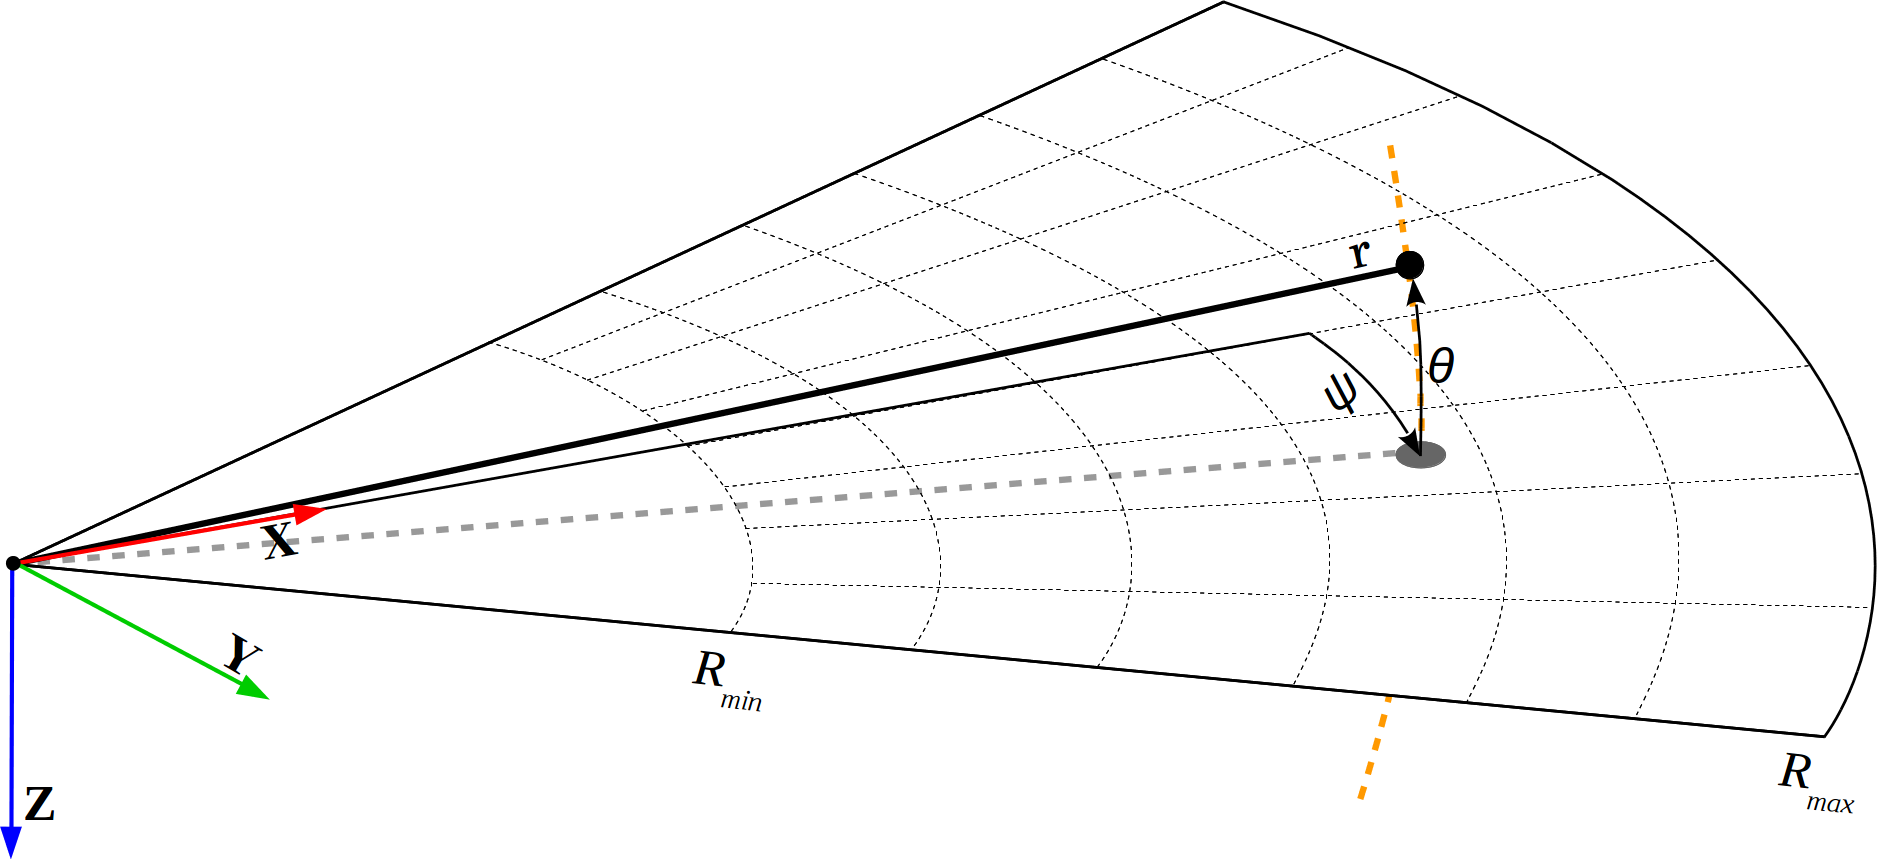
\includegraphics[width=\columnwidth]{figs/sonar_geometry_2}
    \centering
    \captionsetup{justification=centering}
    \caption{Imaging sonar geometry. By the projection process, all 3D points
    belonging to the same elevation arc (represented as dashed red line) will
    be represented to the same image point in the 2D plane. This way,
    range $r$ and azimuth angle $\psi$ are measured, and elevation
    angle $\theta$ is lost. The sonar covered area is defined by $R_{min}$
    and $R_{max}$.}
    \label{fig:sonar_geometry}
\end{figure}

% ----------------------------------------------------------------------------------

\subsection{Sonar characteristics}
\label{sonar:characteristics}

Although sonar devices overcome the main limitations of optical sensors, they
present more difficult data interpretation due to:

\begin{enumerate}[(a)]
    \item \textbf{Shadowing}: This effect is caused by objects blocking the
    sound waves transmission and causing regions behind, without acoustic
    feedback. These regions are defined by a black spot in the image
    occluding part of the scene;
    \item \textbf{Non-uniform resolution}: The amount of pixels used to
    represent an intensity record in the cartesian coordinate system grows as
    its range increases. This fact causes image distortions and object flatness;
    \item \textbf{Changes in viewpoint}: Imaging the same scene from different
    viewpoints can cause occlusions, shadows movements and significant
    alterations of observable objects \cite{hurtos2014}. For instance, when an
    outstanding object is insonified, its shadow is shorter, as the sonar
    becomes closer;
    \item \textbf{Low signal-to-noise ratio (SNR)}: The sonar suffers from low
    SNR mainly due the very-long-range scanning, and the presence of speckle
    noise introduced caused by acoustic wave interferences \cite{abbott1979};
    \item \textbf{Reverberation}: This phenomena is caused when multiple acoustic
    waves returning from the same object are detected over the same ping,
    producing duplicated objects.
\end{enumerate}

% ----------------------------------------------------------------------------------
\begin{figure*}[t]
    \centering
    \subfigure[][]{
    	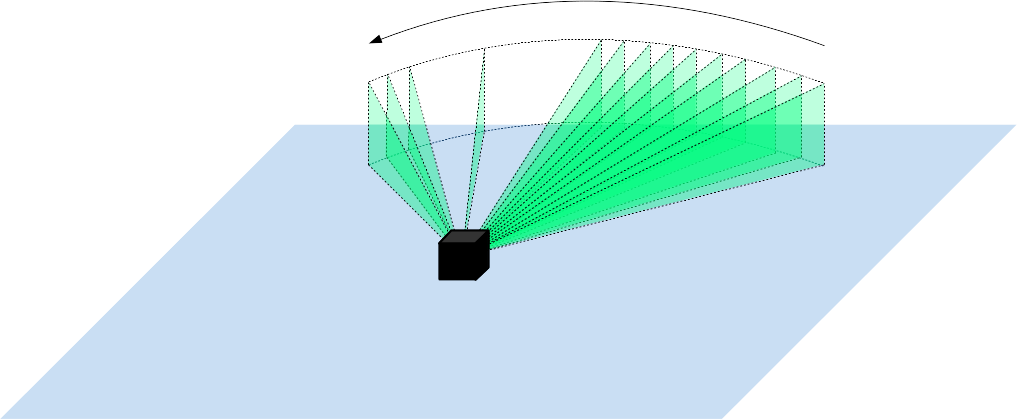
\includegraphics[width=\columnwidth]{figs/sonar_swarths_msis_2}
        \label{fig:swarths:msis}
    }
    \subfigure[][]{
    	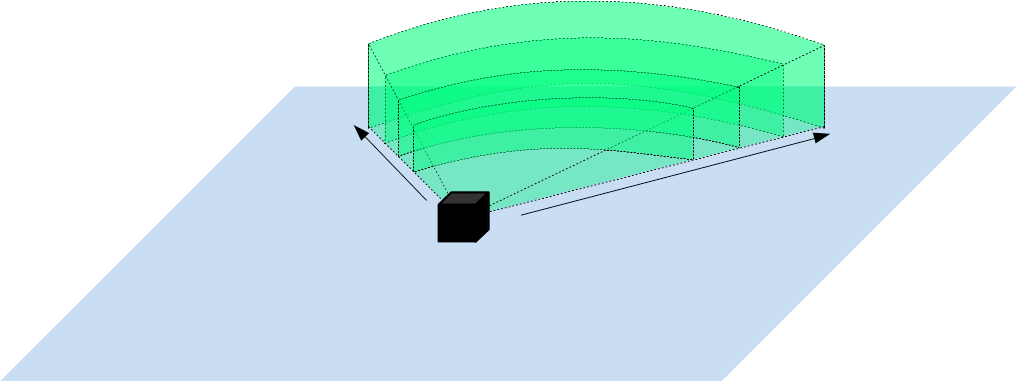
\includegraphics[width=\columnwidth]{figs/sonar_swarths_fls_2}
        \label{fig:swarths:fls}
    }
    \captionsetup{justification=centering}
    \caption{Different underwater sonar readings: \subref{fig:swarths:msis}
    From a mechanical scanning imaging sonar and \subref{fig:swarths:fls}
    from a forward-looking sonar.}
    \label{fig:sonar_devices}
\end{figure*}

\subsection{Types of underwater sonar devices}
\label{sonar:devices}

The most common types of underwater acoustic sonars are MSIS and FLS. In
the former, the sonar image is built for each pulse, with one beam per
reading (see Fig. \ref{fig:swarths:msis}); these sonar images are usually
shown on a display pulse by pulse, and the head position reader is rotated
according to motor step angle. After a full $360^{\circ}$ sector reading
(or the desired sector defined by left and right limit angles), the
accumulated sonar data is overwritten. The acquisition of a scanning image
involves a relatively long time, introducing distortions caused by the
vehicle movements. This sonar device is generally applied in obstacle
avoidance \cite{ganesan2015} and navigation \cite{ribas2010} applications.

As illustrated in Fig. \ref{fig:swarths:fls}, the whole forward view of an
FLS is scanned and the current data is overwritten by the next one in a high
frame rate, with \textit{n} beams being read simultaneously. This is similar
to a streaming video imagery for real-time applications. This imaging sonar
is commonly used for navigation \cite{fallon2013},
mosaicing \cite{hurtos2014}, target tracking \cite{liu2016}
and 3D reconstruction \cite{huang2015}.

% ----------------------------------------------------------------------------------

\begin{figure*}[t]
    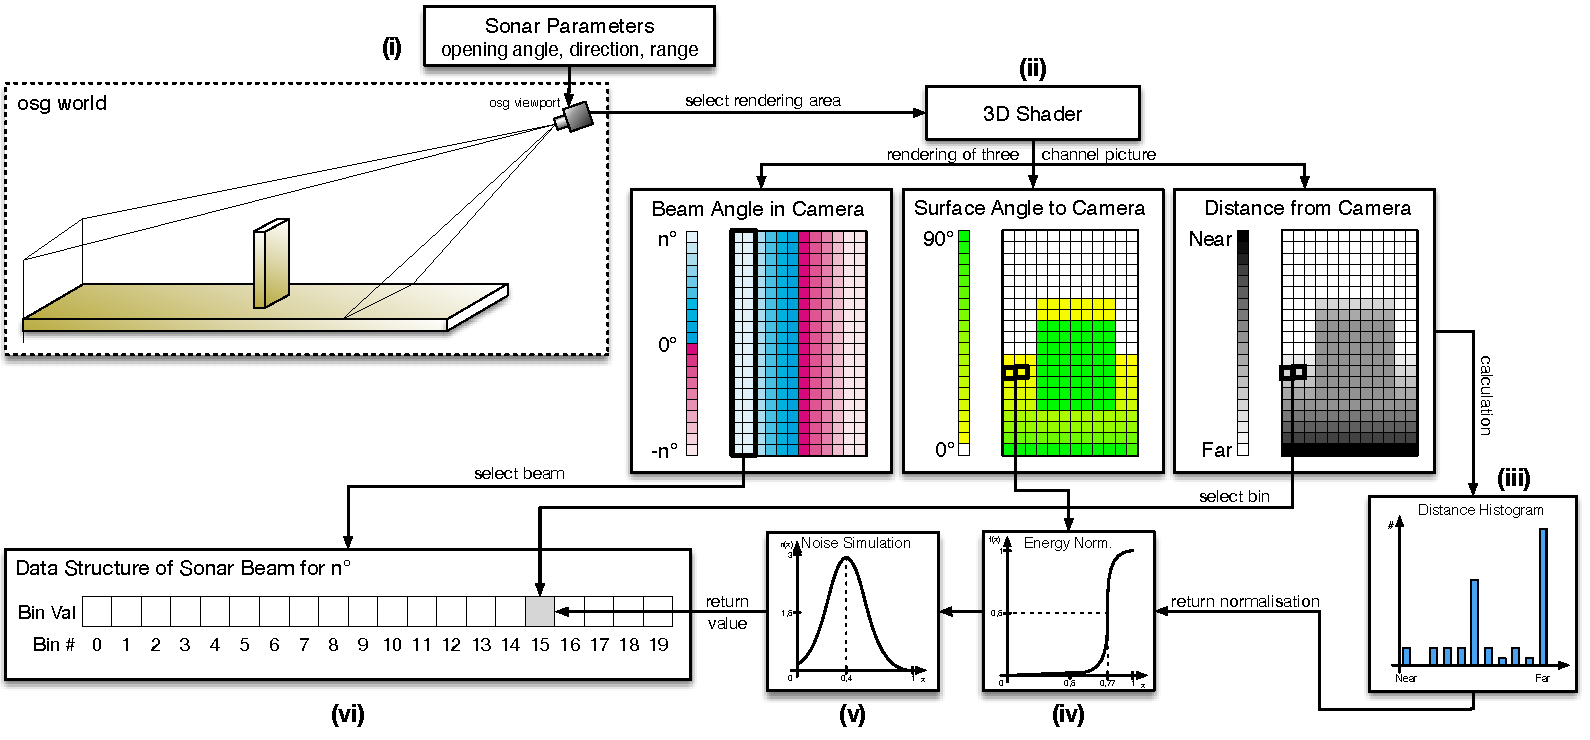
\includegraphics[width=0.85\paperwidth]{figs/sonar_sim}
    \centering
    \captionsetup{justification=centering}
    \caption{A graphical overview of the imaging sonar simulation process:
    (i) a virtual camera, specialized as the sonar device, samples the
    underwater scene; (ii) three components are calculated by shader
    rendering on GPU: The Euclidean distance from camera center, the surface
    normal angles, and the angular distortion; the shader information is
    splitted in beam parts, according the angular distortion values, and
    bin depth and intensity are defined by distance histogram (iii) and energy
    normalization (iv); (v) the speckle noise is added to the final sonar data;
    (vi) the simulated data is presented as Rock's data type.}
    \label{fig:sonar_sim}
\end{figure*}


% ----------------------------------------------------------------------------------

\section{GPU-based sonar simulation}
\label{dev}

The goal of this work is to simulate two types of underwater sonar by vertex
and fragment processing, with a low computational cost. The complete pipeline
of the proposed simulator, from the virtual scene to the simulated acoustic data,
is seen in Fig. \ref{fig:sonar_sim} and is detailed in the following subsections.
The sonar simulation is written in C++ with OpenCV \cite{bradski2000} support as
Rock packages.

% ----------------------------------------------------------------------------------

\subsection{Rendering underwater scene}
\label{dev:uwscene}

The Rock-Gazebo integration \cite{watanabe2015} provides the underwater
scenario, and allows real-time hardware-in-the-loop simulations. In this
framework, Gazebo handles the physical engines, and the Rock's visualization
tools are responsible by the scene rendering. The graphical data in Rock are
based on OpenSceneGraph framework, an open source C/C++ 3D graphics toolkit
built on OpenGL. The osgOcean framework is used to simulate the ocean visual
effects, and the ocean buoyancy is defined by the Gazebo, as described
in \cite{watanabe2015}.

All scene aspects, such as world model, robot parts (including sensors and
joints) and other objects presented in the environment are defined by simulation
description files (SDF), which use the SDFormat \cite{sdformat2017}, a XML
format used to describe simulated models and environments for Gazebo. Visual
and collision geometries of vehicle and sensor robot are also described in
specific file formats. Each component described in the SDF file becomes a
Rock component, which is based on the Orocos real-time toolkit (RTT)
\cite{soetens2005}, providing I/O ports, properties and operations as
communication layers. When the models are loaded, Rock-Gazebo creates I/O
ports to allow real-world or simulated system components interacting with the
simulated models. A resulting scene sample of this integration is seen
in Fig. \ref{fig:uwscene}.

\begin{figure}[t]
    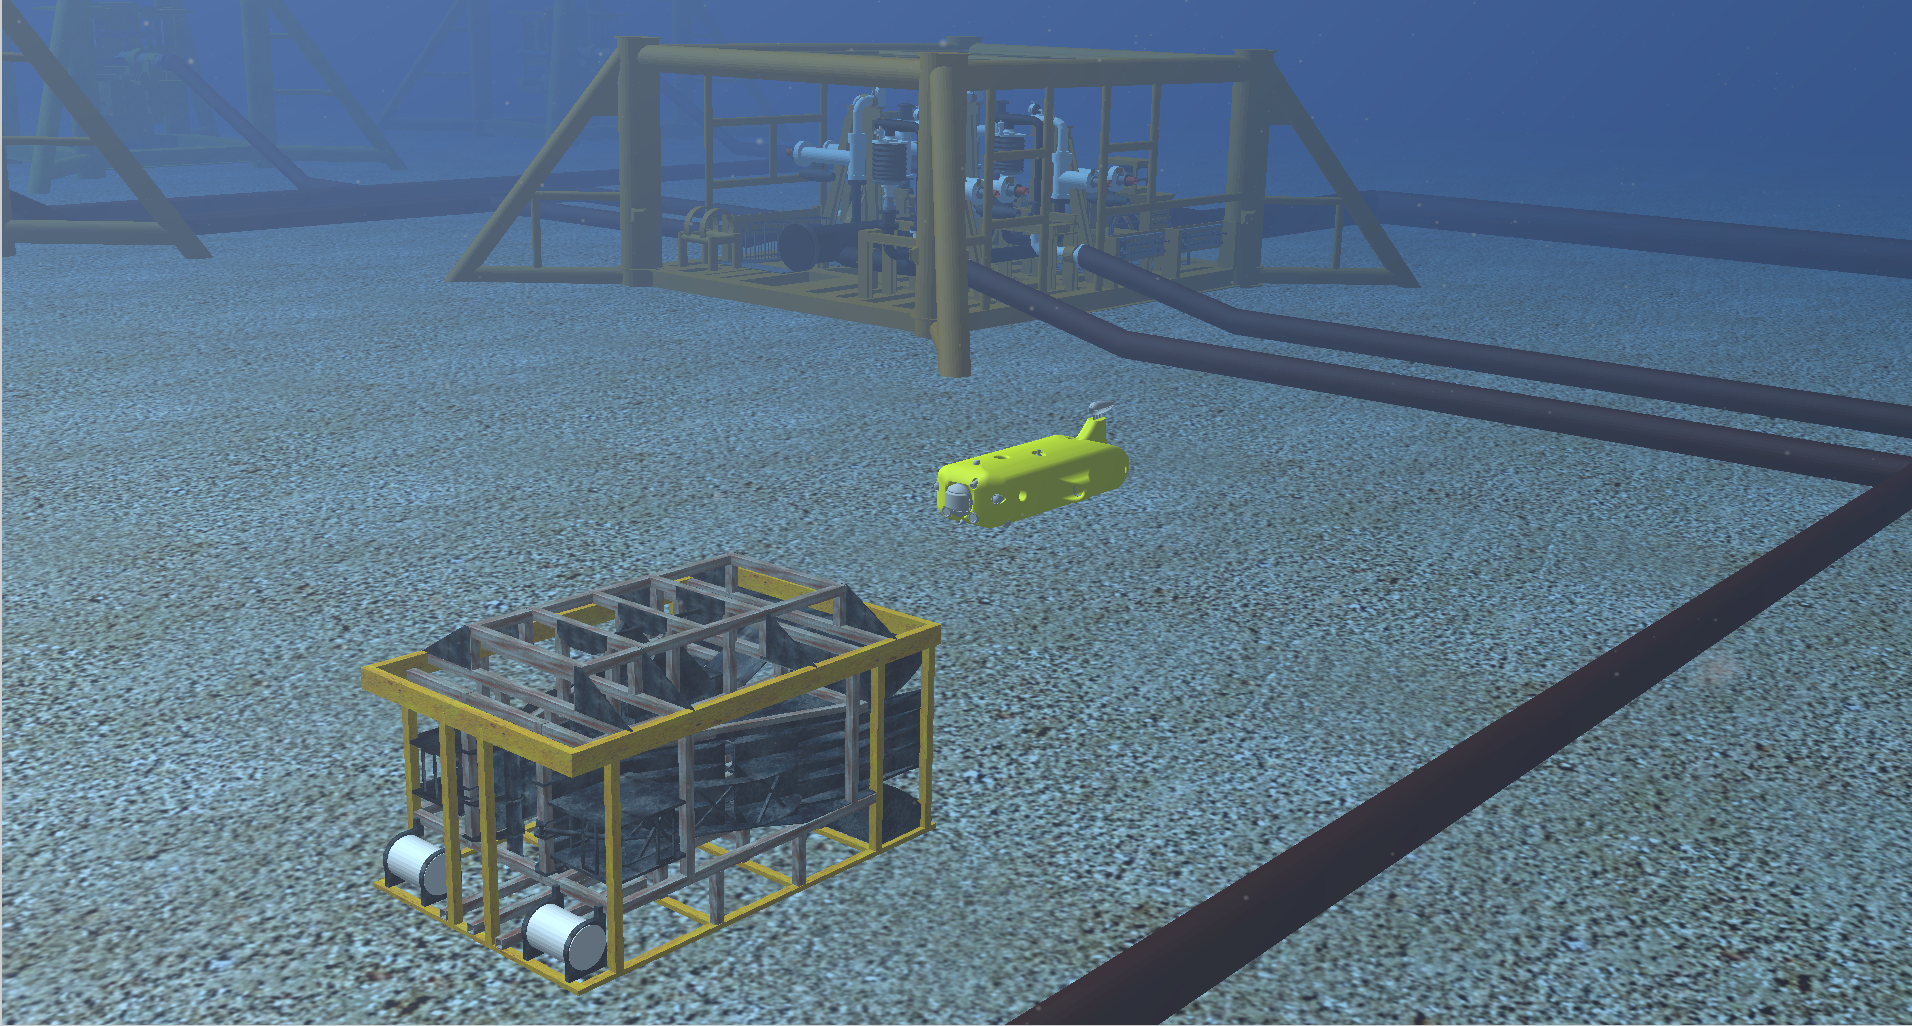
\includegraphics[width=\columnwidth]{figs/uwscene}
    \centering
    \captionsetup{justification=centering}
    \caption{The AUV in Rock-Gazebo underwater scene.}
    \label{fig:uwscene}
\end{figure}

% ----------------------------------------------------------------------------------

\subsection{Shader rendering}
\label{dev:shader}

Modern graphics hardware presents programmable tasks embedded in GPU. Based
on parallel computing, that approach can speed up 3D graphics processing,
reducing the computational effort of the central processing unit (CPU). The
rendering pipeline can be customized by defining programs on GPU called
shaders. A shader is written in OpenGL Shading Language (GLSL) \cite{rost2009},
a high-level language with a C-based syntax which enables more direct control
of graphics pipeline, which avoids the use of low-level or hardware-specific
languages. Shaders can describe the characteristics of either a vertex or a
fragment (a single pixel). Vertex shaders are responsible by transforming the
vertex position into a screen position by the rasterizer, generating texture
coordinates for texturing, and lighting the vertex to determine each color.
The rasterization results in a set of pixels to be processed by fragment
shaders, which manipulate their locations, depth and alpha values, and
interpolated parameters from the previous stages, such as colors and textures.

In our work, the underwater scene is sampled by a virtual camera, whose
optical axis is aligned with the intended viewing direction of the
imaging sonar device, as well as the covered range and opening angle.
By programming the fragment and vertex shaders, the sonar data is
computed as:

\begin{itemize}[(a)]
    \item \textbf{Depth} is the camera focal length, calculated by the
    Euclidean distance to the object surface point;
    \item \textbf{Intensity} presents the echo reflection energy based
    on object surface normal angle up to the camera;
    \item \textbf{Angular distortion} is the angle formed from the camera
    center column up to the camera boundary column, for both directions.
\end{itemize}

All those three informations are normalized into the interval [0,1],
where zero means no energy and one means maximum echo energy for
intensity data, respectively. For depth data, the minimum value portrays
a close object while the maximum value represents a far one, limited by
the sonar maximum range. Angle distortion value is zero in image center
column which increases for both borders to present the half value
of horizontal field of view.

In realistic sensing, real-world surfaces usually present irregularities
and different reflectance values. To render that in a virtual scene, the
intensity values can also be defined by a normal maps and material
property information. Normal mapping is a perturbation rendering technique
to simulate wrinkles and dents on the object surface by passing RGB textures and modifying
the normal directions on shaders. This approach consumes less computational
resources for the same level of detail, compared to the displacement mapping
technique, because the geometry remains unchanged. Since normal maps are
built in tangent space, interpolating the normal vertex and the texture,
a tangent, bitangent and normal (TBN) matrices are computed to convert the
normal values into the world space. Representation of normal mapping process
in our approach is seen in Fig. \ref{fig:sonar_normal_mapping}.

\begin{figure*}[t]
    \centering
    \subfigure[][]{
        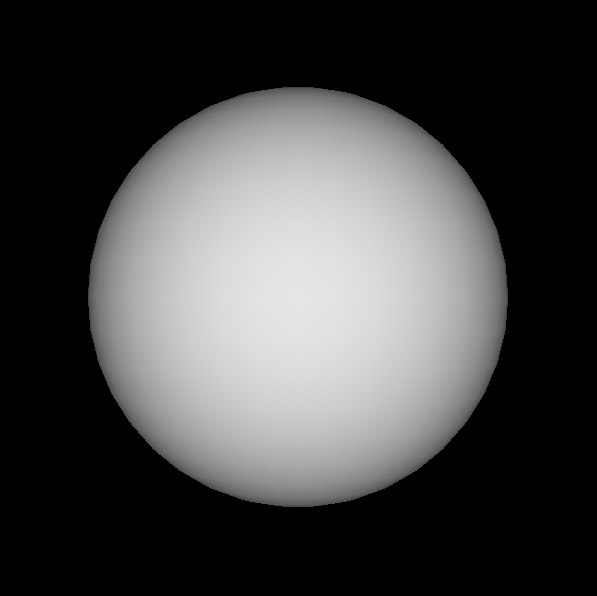
\includegraphics[width=0.25\paperwidth]{figs/normal_map_0}
        \label{fig:normal_0}
    }
    \subfigure[][]{
        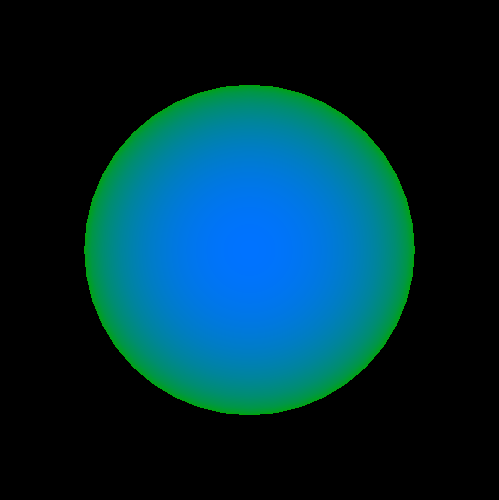
\includegraphics[width=0.25\paperwidth]{figs/normal_map_1}
        \label{fig:normal_1}
    }
    \subfigure[][]{
        
\includegraphics[width=0.25\paperwidth]{figs/normal_map_2}
        \label{fig:normal_2}
    }
    \subfigure[][]{
        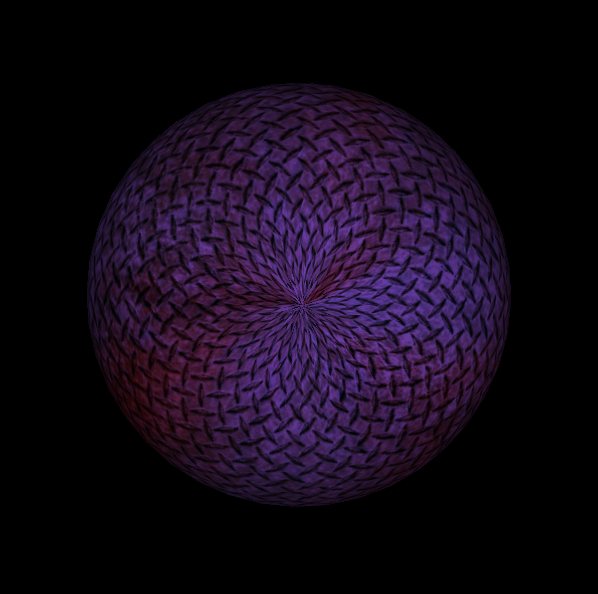
\includegraphics[width=0.25\paperwidth]{figs/normal_map_3}
        \label{fig:normal_3}
    }
    \subfigure[][]{
        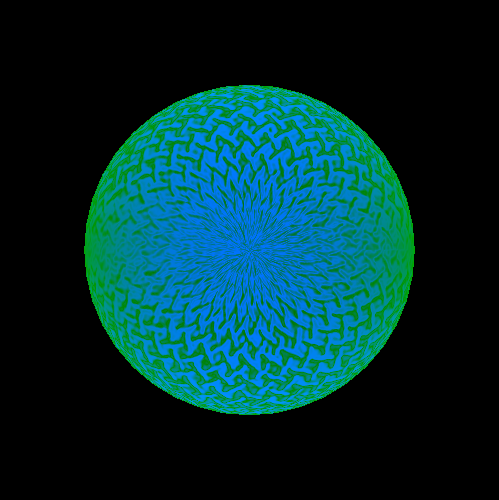
\includegraphics[width=0.25\paperwidth]{figs/normal_map_4}
        \label{fig:normal_4}
    }
    \subfigure[][]{
        
\includegraphics[width=0.25\paperwidth]{figs/normal_map_5}
        \label{fig:normal_5}
    }
    \captionsetup{justification=centering}
    \caption{Example of shader rendering with normal mapping processing:
    A sphere without texture \subref{fig:normal_0} and with texture
    \subref{fig:normal_3}; their respective shader image representation
    in \subref{fig:normal_1} and \subref{fig:normal_4}, where blue is the
    normal channel and green is the depth one; and the final acoustic
    image in \subref{fig:normal_2} and \subref{fig:normal_5}. By using
    normal mapping technique, the textures changes the normal directions,
    and the sonar image details the appearance of object surface, like
    in real-world sensing.}
    \label{fig:sonar_normal_mapping}
\end{figure*}

The reflectance allows to properly describe the intensity received back
from observable objects in shader processing, according their material
properties. For instance, aluminum has more reflectance than wood and
plastic. When an object has its reflectivity defined, the reflectance
value $\rho$ is passed to fragment shader and must be positive. As seen
in Fig. \ref{fig:sonar_reflectances}, normal values are directly
proportional to the reflectance value $\rho$. At the end, the shader process
provides a matrix with three main data: Intensity, depth and
angular distortion.

\begin{figure}[h]
    \centering
    \subfigure[][]{
    	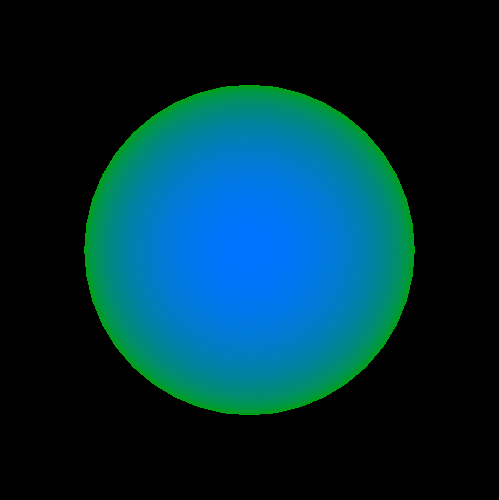
\includegraphics[width=0.45\columnwidth]{figs/reflectance_0}
        \label{fig:reflectance:0}
    }
    \subfigure[][]{
    	
\includegraphics[width=0.45\columnwidth]{figs/reflectance_0_35}
        \label{fig:reflectance:0.35}
    }
    \subfigure[][]{
    	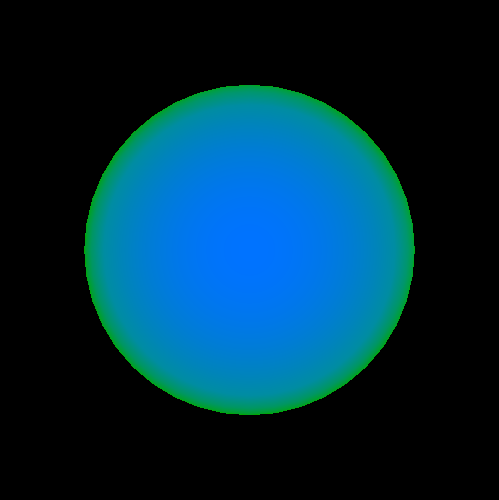
\includegraphics[width=0.45\columnwidth]{figs/reflectance_1_40}
        \label{fig:reflectance:1.40}
    }
    \subfigure[][]{
    	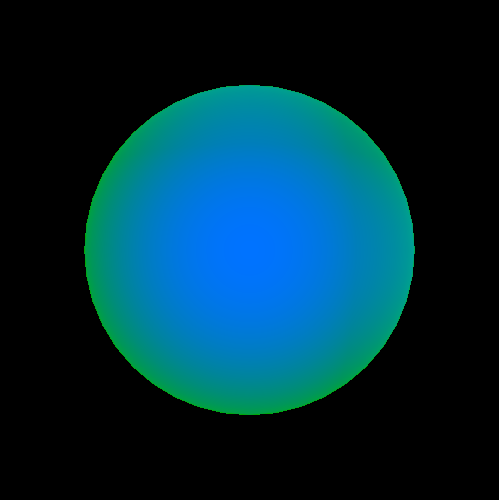
\includegraphics[width=0.45\columnwidth]{figs/reflectance_2_12}
        \label{fig:reflectance:2.12}
    }
    \captionsetup{justification=centering}
    \caption{Examples of different reflectance values, $\rho$, applied in
    shader image representation, where blue is the normal channel and
    green is the depth channel: \subref{fig:reflectance:0} raw image;
    \subref{fig:reflectance:0.35} $\rho = 0.35$;
    \subref{fig:reflectance:1.40} $\rho = 1.40$; and
    \subref{fig:reflectance:2.12} $\rho = 2.12$.}
    \label{fig:sonar_reflectances}
\end{figure}


% ----------------------------------------------------------------------------------

\subsection{Simulating sonar device}
\label{dev:sonardata}

The 3D shader matrix is processed in order to build the corresponding
acoustic representation. Since the angular distortion is radially spaced
over the horizontal field-of-view, where all pixels in the same column
have the same angle value, the first step is to split the image in a
number of beam parts. Each column is correlated with its respective beam,
according to sonar bearings, as seen in Fig. \ref{fig:sonar_sim}. Each
beamed sub-image is converted into bin intensities using the depth and
intensity data. In a real imaging sonar, the echo measured back is sampled
over time and the bin number is proportional to the sensor range. In other
words, the initial bins represent the closest distances, while the latest
bins are the farthest ones. Therefore a distance histogram is evaluated to
group the sub-image pixels with their respective bins, according to the
depth value. This information is used to calculate the accumulated
intensity of each bin.

Due to the acoustic beam spreading and absorption in the water, the final
bins have less echo strength than the first ones, because the energy is
lost twice, in the environment. To tackle with that issue, the sonar devices
use an energy normalization based on time-varying gain for range dependence
compensation, which spreads losses in the bins. In our simulation approach,
the accumulated intensity in each bin is normalized as

\begin{equation}
    \label{eq:1}
    I_{bin} = \sum\limits_{x=1}^N \frac{1}{N} \times S(i_{x}) \, ,
\end{equation}
where $I_{bin}$ is the intensity in the bin after energy normalization,
$x$ is the pixel location in the shader matrix, $N$ is the depth histogram
value (number of pixels) of that bin, $S(i_{x})$ is a sigmoid function,
and $i_{x}$ is the intensity value of the pixel $x$.

Finally, the sonar image resolution needs to be big enough to fill all
informations of the bins. For that, the number of bins involved is in direct
proportion to the sonar image resolution.

% ----------------------------------------------------------------------------------

\subsection{Noise model}
\label{dev:noise}

Imaging sonar systems are disturbed by a multiplicative noise known as speckle,
and caused by coherent processing of backscattered signals from multiple
distributed targets. These latter ones degrade image quality and the visual
evaluation. Speckle noise results in constructive and destructive interferences
which are shown as bright and dark dots in the image. The noisy image has been
expressed as \cite{lee1980}:

\begin{equation}
\label{eq:2}
y(t) = x(t) \times n(t) \, ,
\end{equation}
where $t$ is the time instant, $y(t)$ is the noised image, $x(t)$ is the
free-noise image, $n(t)$ is the speckle noise matrix, and $\times$ symbol defines an
element-wise multiplication.

This type of noise is well-modeled as a Gaussian distribution. The physical
explanation is provided by the central limit theorem, which states that the
sum of many independent and identically distributed random variables tends
to behave a Gaussian random variable. A Gaussian distribution is defined
by following a non-uniform distribution, skewed towards low values, as seen
in Fig. \ref{fig:sonar_sim}, and applied as speckle noise in the simulated
sonar image. After that, the simulation sonar data process is performed in
each frame.

\subsection{Integrating sonar device with Rock}
\label{dev:rock}

To export and display the sonar image, the simulated data is encapsulated
as Rock's sonar data type, and provided as an output I/O port of a Rock's
component.

% ----------------------------------------------------------------------------------

\section{Simulation results and experimental analysis}
\label{results}

To evaluate our simulator, experiments were conducted by using a 3D model
of an AUV equipped with one MSIS and one FLS, studied in different scenarios.
The following devices configuration are summarized in
Table \ref{table:sonar_settings}. As the scene frames are being captured by
the sonars, resulting simulated acoustic images are sequentially presented,
on-the-fly.

\subsection{Experimental evaluation}

The virtual FLS from AUV was used to insonify the scenes from three distinct
scenarios. A docking station, in parallel with a pipeline on the seabed,
composes \textbf{the first scenario} (see Fig. \ref{fig:fls_scene1}). The
target surface is well-defined in the simulated acoustic frame (see
Fig. \ref{fig:fls_sim1}), even as the shadows and speckle noise. Given the
docking station is metal-made, the texture and reflectivity were set, such
as a higher intensity shape was resulted in comparison with the other targets.
\textbf{The second scenario} presents the vehicle in front of a manifold model
in a non-uniform seabed (see Fig. \ref{fig:fls_scene2}). The target model was
insonified to generate the sonar frame from the underwater scene. The frontal
face of the target, as well the portion of the seabed and the degraded data
by noise, are clearly visible in the FLS image. Also, a long acoustic shadow
is formed behind the manifold, occluding part of the scene. \textbf{The
third scenario} contains a sub-sea isolation valve (SSIV) structure, connected
to a pipeline in the bottom (see Fig. \ref{fig:fls_scene3}).

\begin{table}[t]
    \caption{Sonar devices configurations used on experimental evaluation.}
    \label{table:sonar_settings}
    \begin{center}
        \begin{tabular}{| c | c | c | c | c | c |}
            \hline
            \rule{0pt}{15pt}
            \makecell[c]{Device} & \makecell[c]{\shortstack{\# of\\ beams}} & \makecell[c]{\shortstack{\# of\\ bins}} & \makecell[c]{\shortstack{Field \\of view}} & \makecell[c]{\shortstack{Down\\tilt}} & \makecell{\shortstack{Motor\\Step}}\\
            \hline
            FLS  & 256 & 1000 & $120^{\circ}$ x $20^{\circ}$ & $20^{\circ}$  & - \\ \hline
            MSIS & 1   & 500  & $3^{\circ}$ x $35^{\circ}$	 & $0^{\circ}$  & $1.8^{\circ}$ \\ \hline
        \end{tabular}
    \end{center}
\end{table}

Due to sensor configuration and robot position, the initial bins usually
present a blind region in the three simulated scenes, caused by absence
of objects at lower ranges, similar to real images. Also, the brightness
of sea-floor decreases, when farthest from sonar, because of the normal
orientation of the surface.

\begin{figure*}[!ht]
    \centering
    \subfigure[][]{
        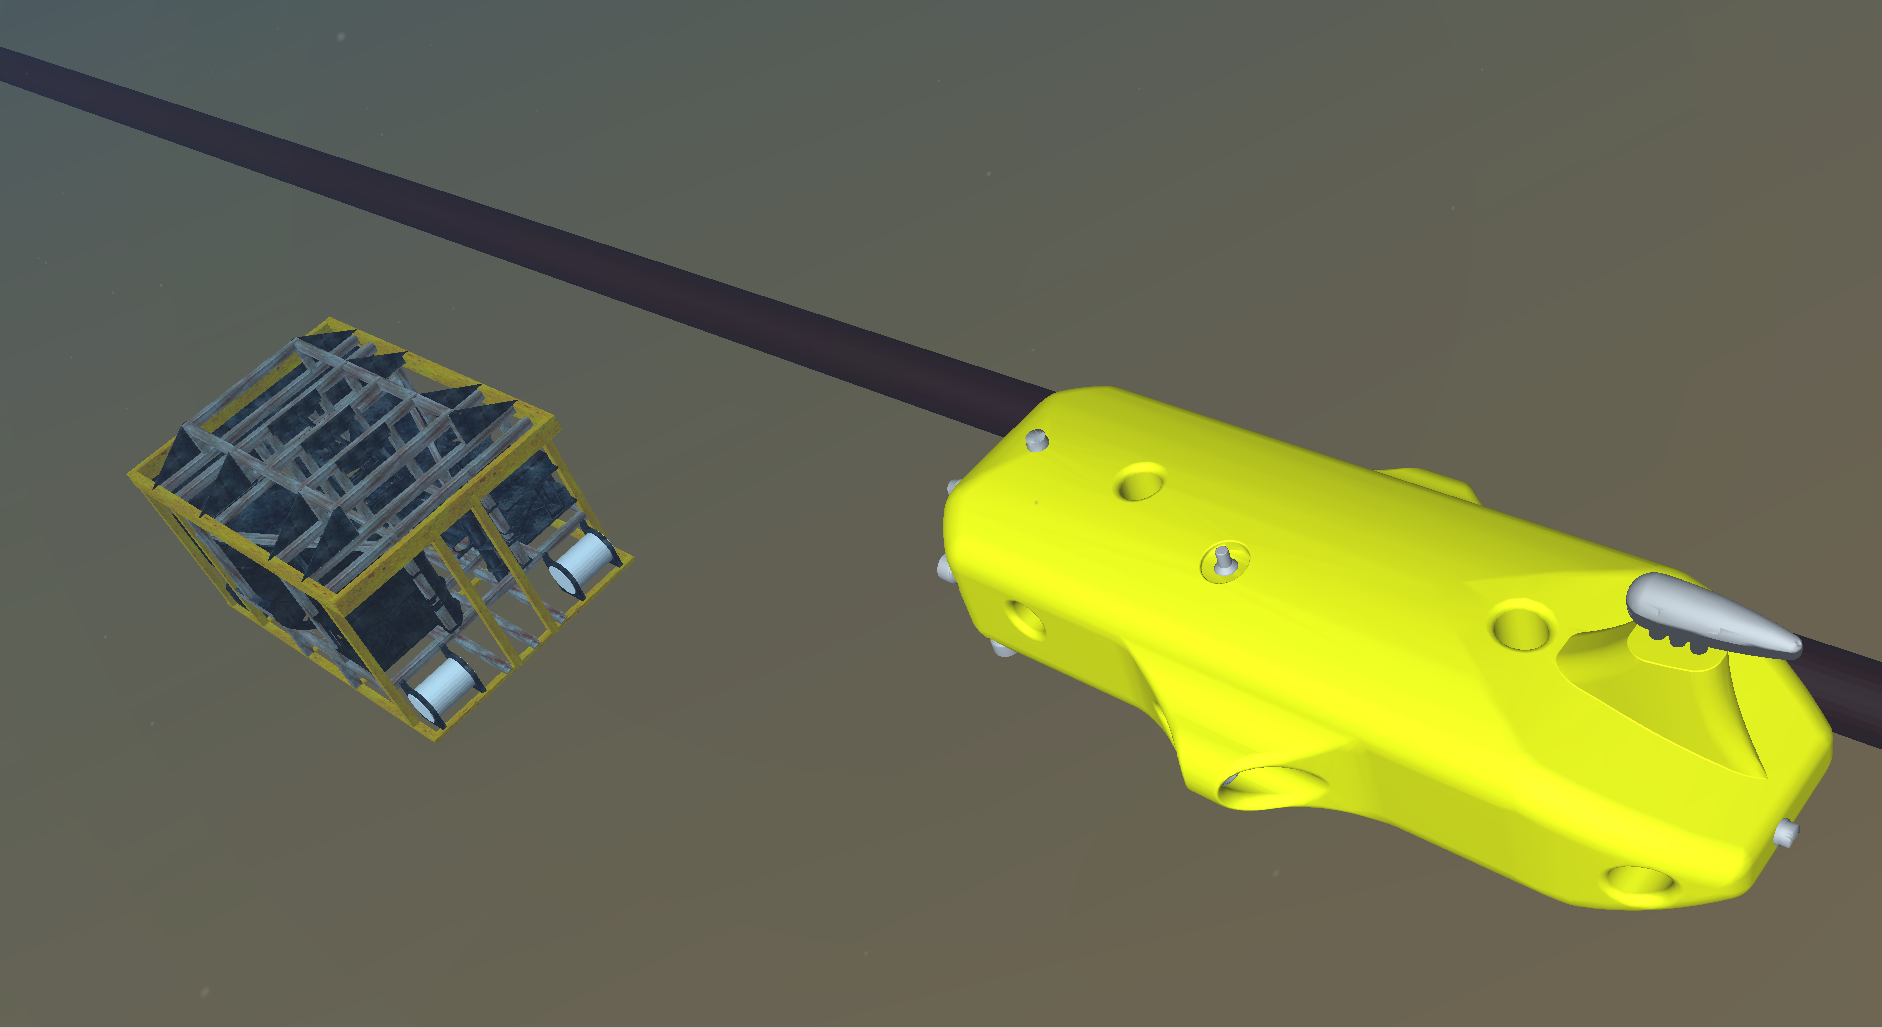
\includegraphics[width=0.4\paperwidth,height=6cm]{figs/fls_scene1}
        \label{fig:fls_scene1}
    }
    \subfigure[][]{
        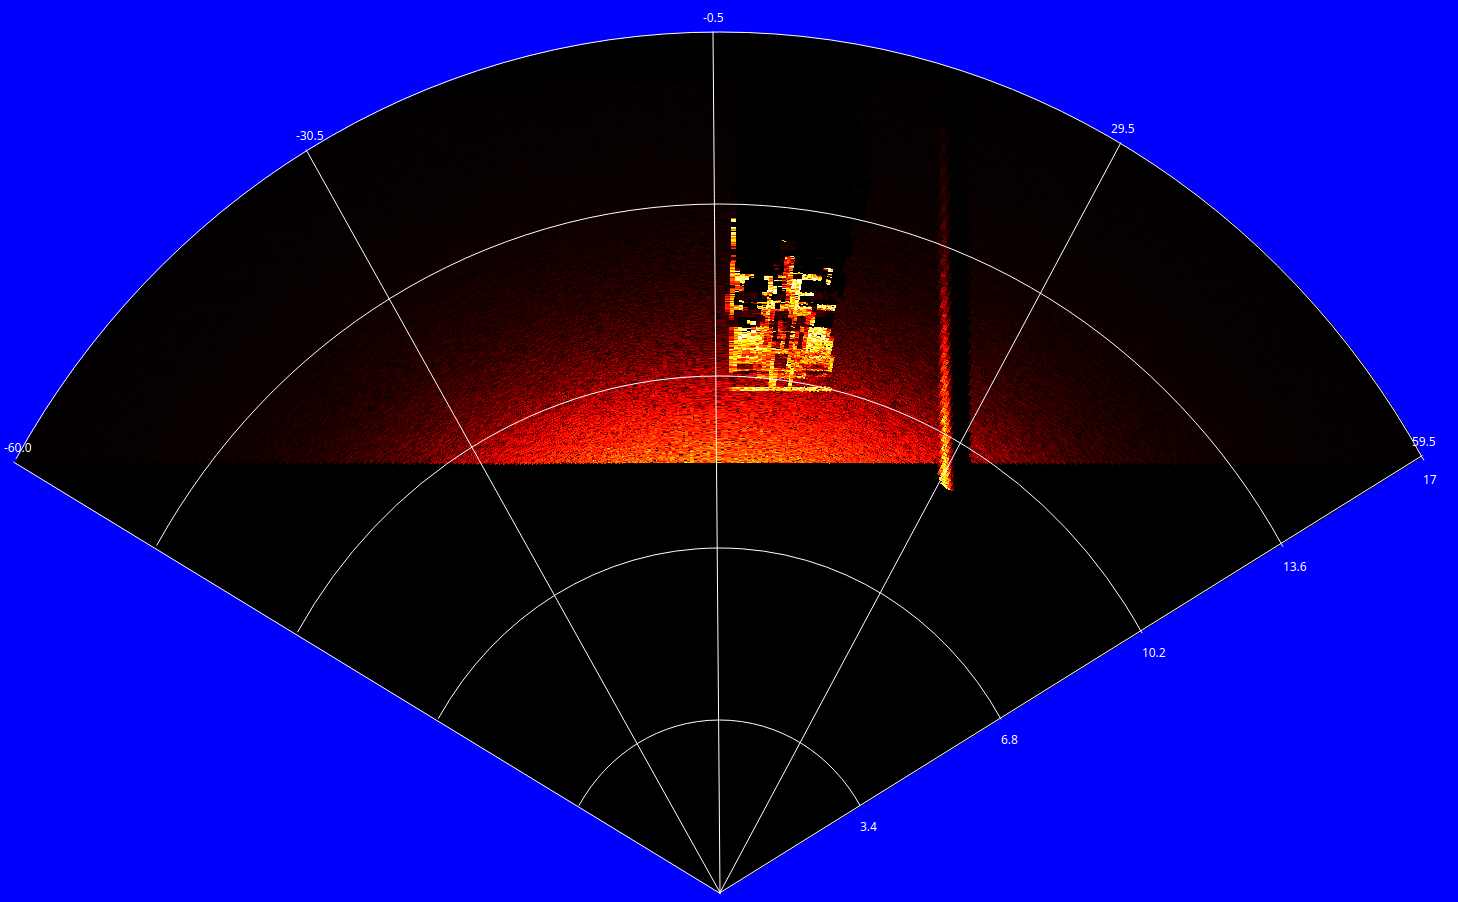
\includegraphics[width=0.4\paperwidth,height=6cm]{figs/fls_sim1}
        \label{fig:fls_sim1}
    }
    \subfigure[][]{
        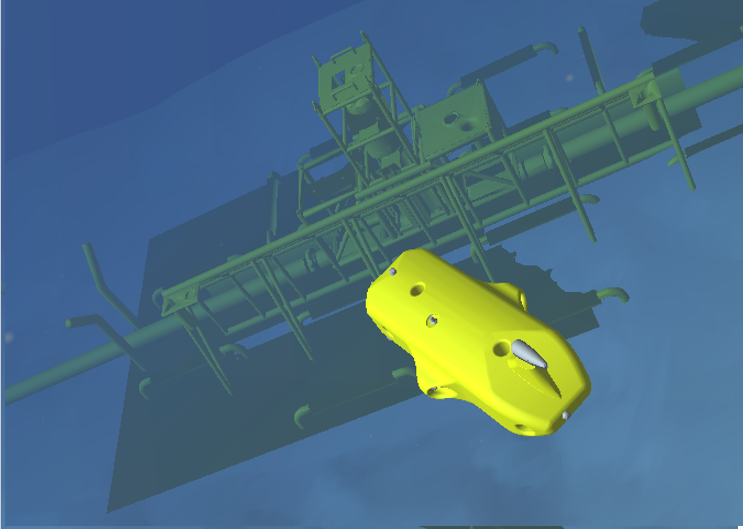
\includegraphics[width=0.4\paperwidth,height=6cm]{figs/fls_scene2}
        \label{fig:fls_scene2}
    }
    \subfigure[][]{
        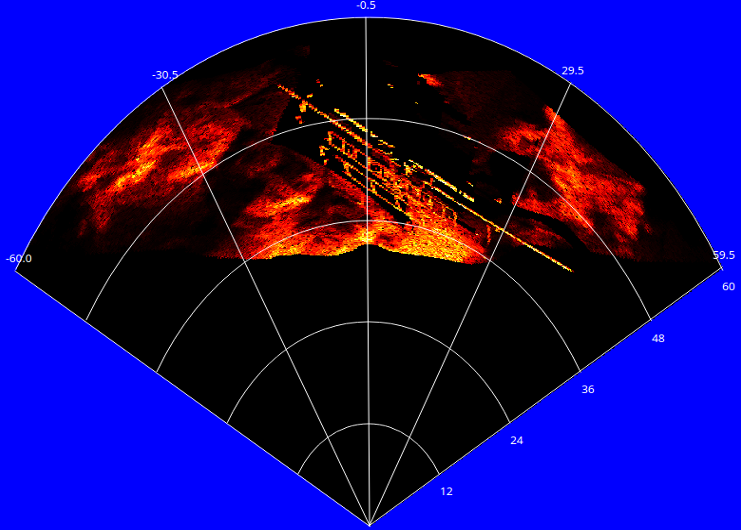
\includegraphics[width=0.4\paperwidth,height=6cm]{figs/fls_sim2}
        \label{fig:fls_sim2}
    }
    \subfigure[][]{
        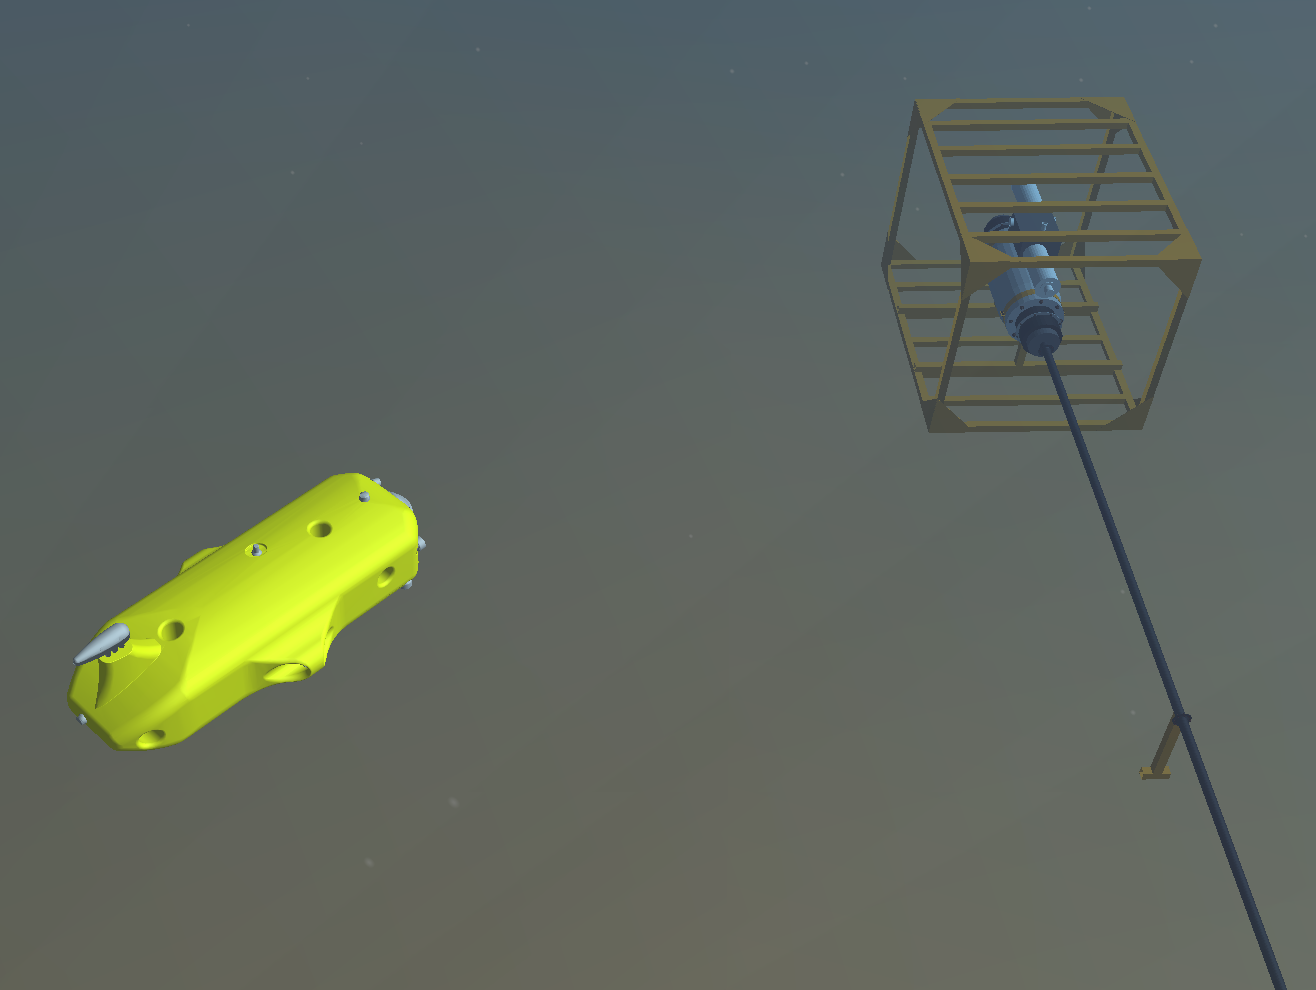
\includegraphics[width=0.4\paperwidth,height=6cm]{figs/fls_scene3}
        \label{fig:fls_scene3}
    }
    \subfigure[][]{
        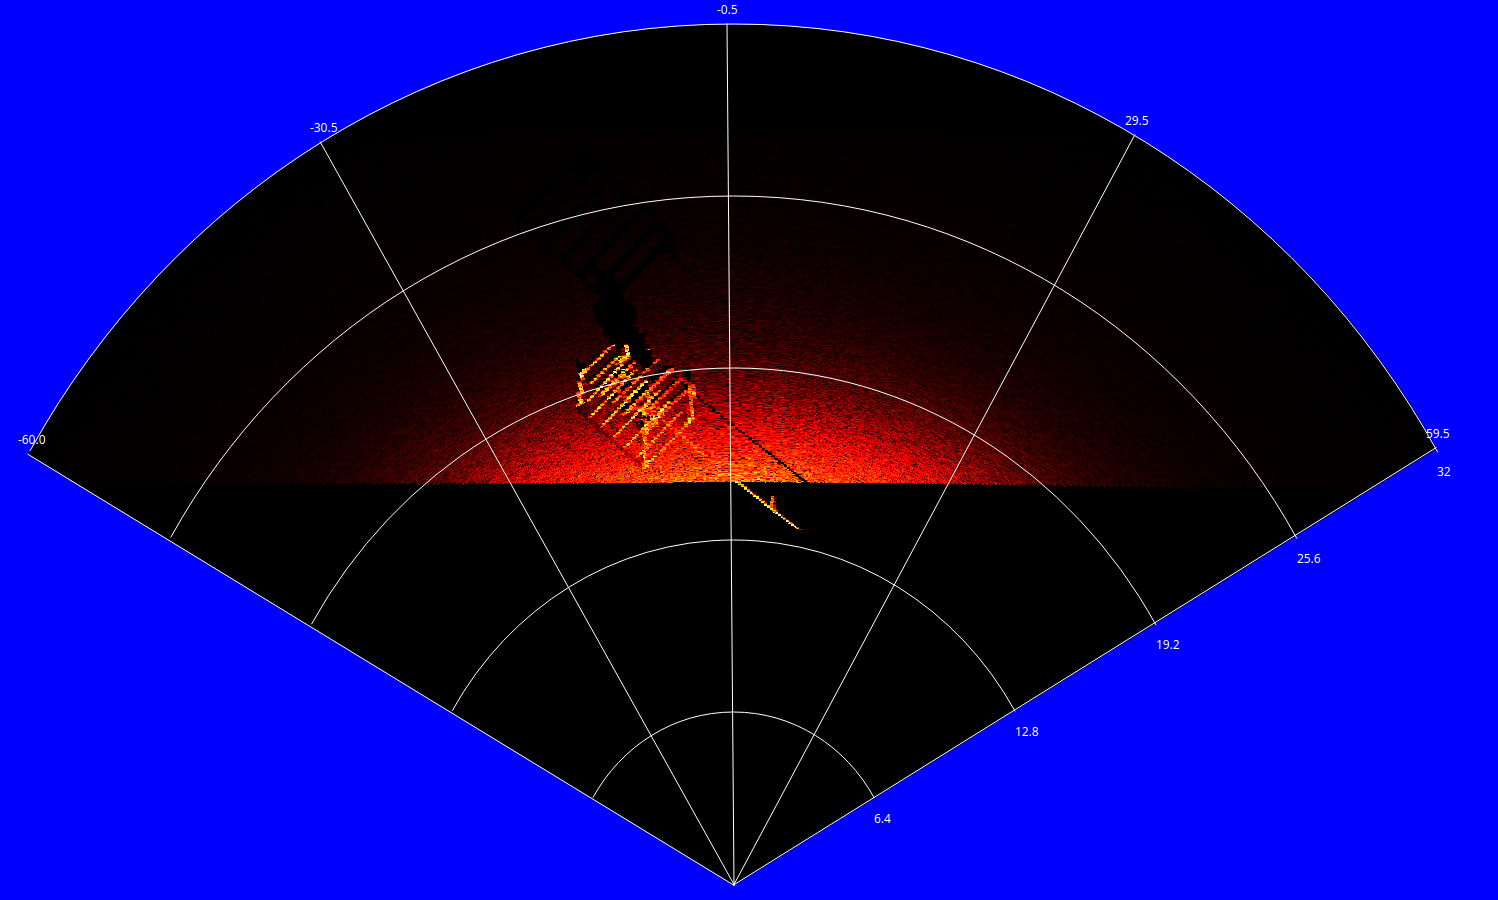
\includegraphics[width=0.4\paperwidth,height=6cm]{figs/fls_sim3}
        \label{fig:fls_sim3}
    }
    \captionsetup{justification=centering}
    \caption{Forward-looking sonar simulation experiments:
    \subref{fig:fls_scene1}, \subref{fig:fls_scene2} and \subref{fig:fls_scene3}
    present the virtual underwater trials, while \subref{fig:fls_sim1},
    \subref{fig:fls_sim2} and \subref{fig:fls_sim3} are the following acoustic
    representations of each scenario, respectively.}
    \label{fig:fls}
\end{figure*}

The MSIS was also simulated in three different experiments. The robot in a
big textured tank composes \textbf{the first scene} (see Fig.
\ref{fig:msis_scene1}). Similar to the first scenario of FLS experiment,
the reflectivity and texture were set to the target. The rotation of the
sonar head position, by a complete $360^{\circ}$ scanning, produced the acoustic
frame of tank walls (see Fig. \ref{fig:msis_sim1}). \textbf{The second scene}
involves the vehicle's movement during the data acquisition process. The scene
contains a grid around the AUV (see Fig. \ref{fig:msis_scene2}), a MSIS in
the front of the AUV is used. This trial induces a distortion in the final
acoustic frame, because the relative sensor position with respect to the
surrounding object changes while the sonar image is being built (see
Fig. \ref{fig:msis_sim2}). In this case, the robot rotates $20^{\circ}$ left
during the scanning. \textbf{The last scene} presents the AUV over oil
and gas structures on the sea bottom (see Fig. \ref{fig:msis_scene3}).
Using a MSIS located in the back of the AUV, with a vertical orientation,
the scene was scanned to produce the acoustic visualization. As illustrated
in Fig. \ref{fig:msis_sim3}, object surfaces present clear definition in
the slice scanning of the sea-floor.

\begin{figure*}[!ht]
    \centering
    \subfigure[][]{
        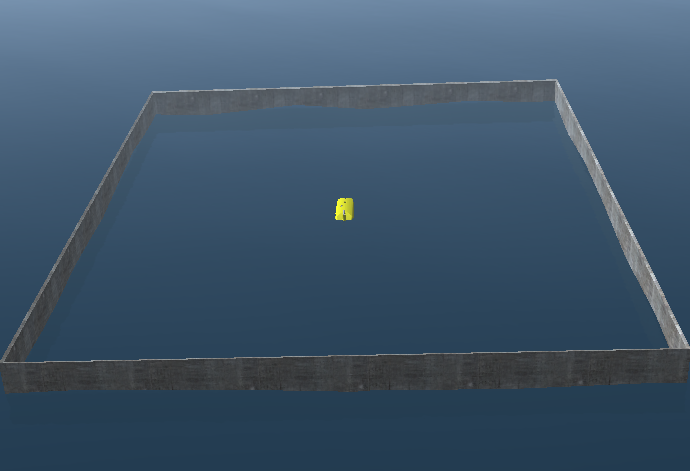
\includegraphics[width=0.4\paperwidth,height=6cm]{figs/msis_scene1}
        \label{fig:msis_scene1}
    }
    \subfigure[][]{
        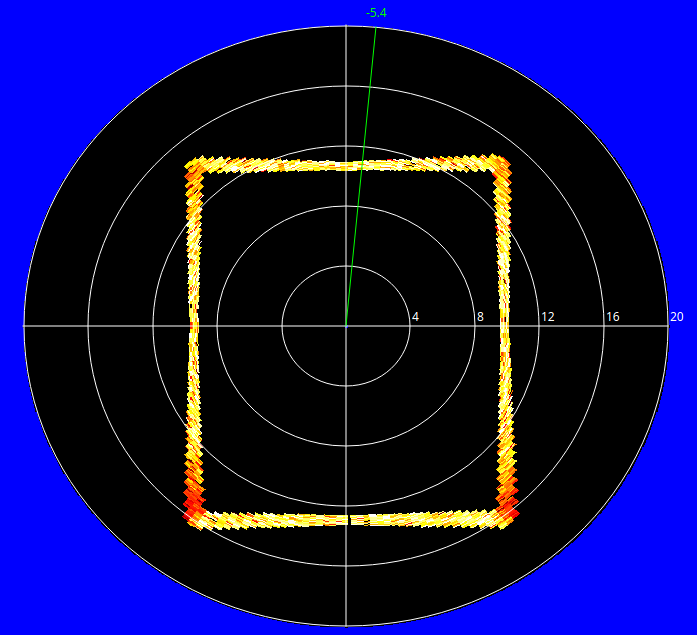
\includegraphics[width=0.4\paperwidth,height=6cm]{figs/msis_sim1}
        \label{fig:msis_sim1}
    }
    \subfigure[][]{
        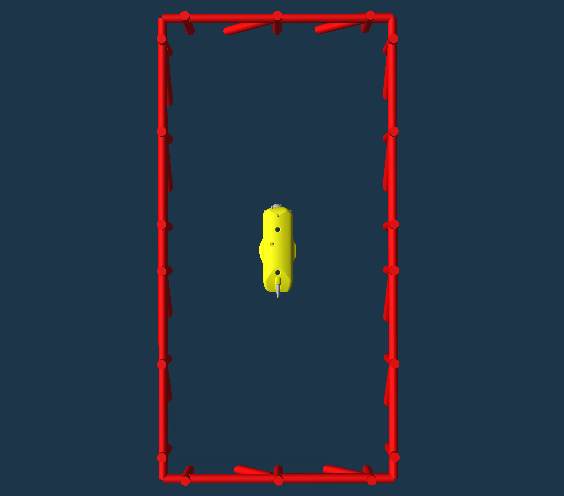
\includegraphics[width=0.4\paperwidth,height=6cm]{figs/msis_scene2}
        \label{fig:msis_scene2}
    }
    \subfigure[][]{
        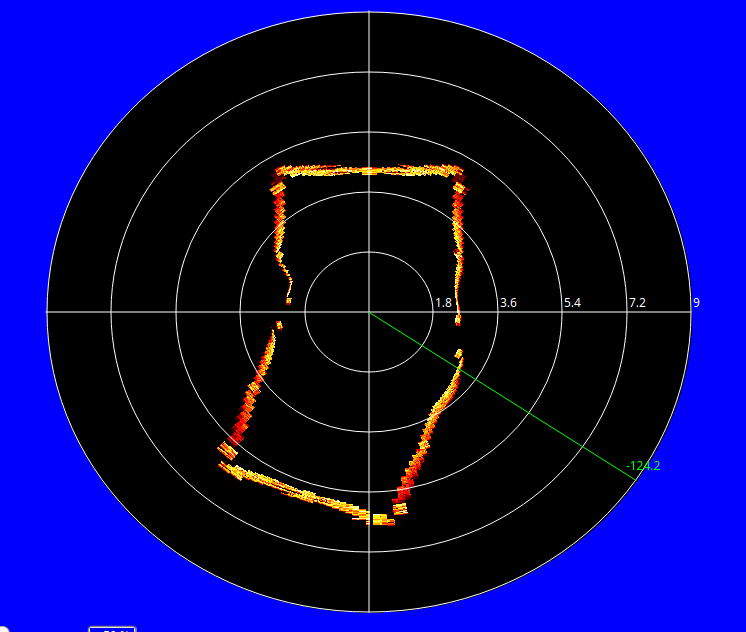
\includegraphics[width=0.4\paperwidth,height=6cm]{figs/msis_sim2}
        \label{fig:msis_sim2}
    }
    \subfigure[][]{
        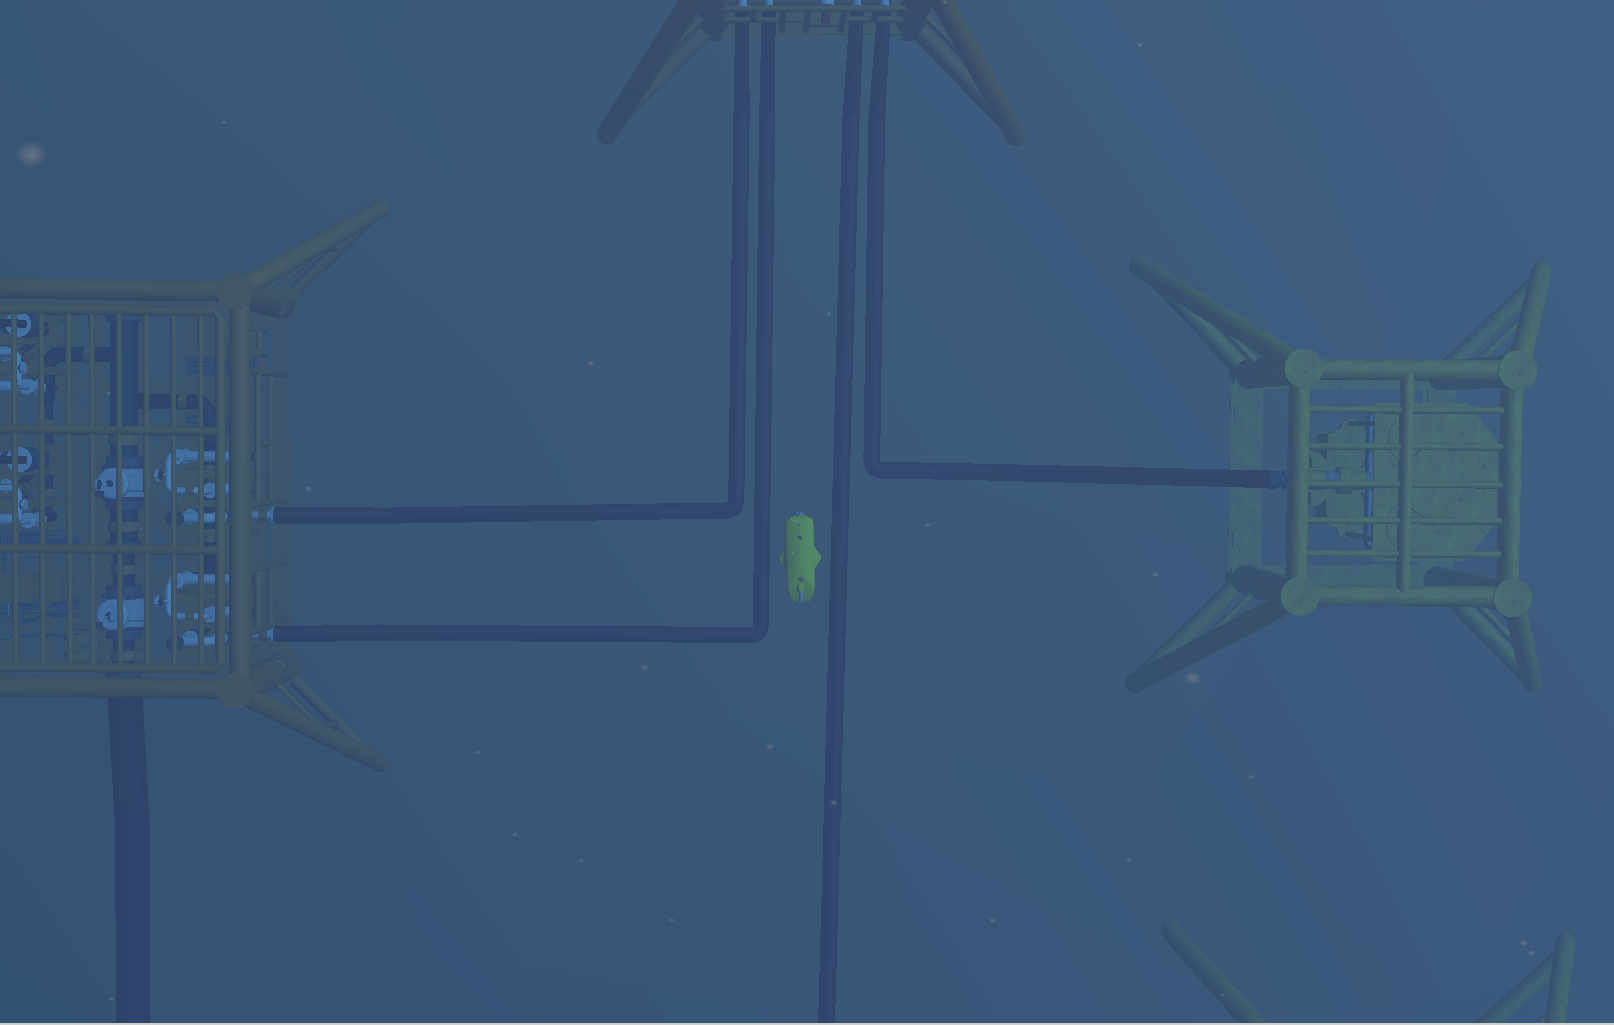
\includegraphics[width=0.4\paperwidth,height=6cm]{figs/msis_scene3}
        \label{fig:msis_scene3}
    }
    \subfigure[][]{
        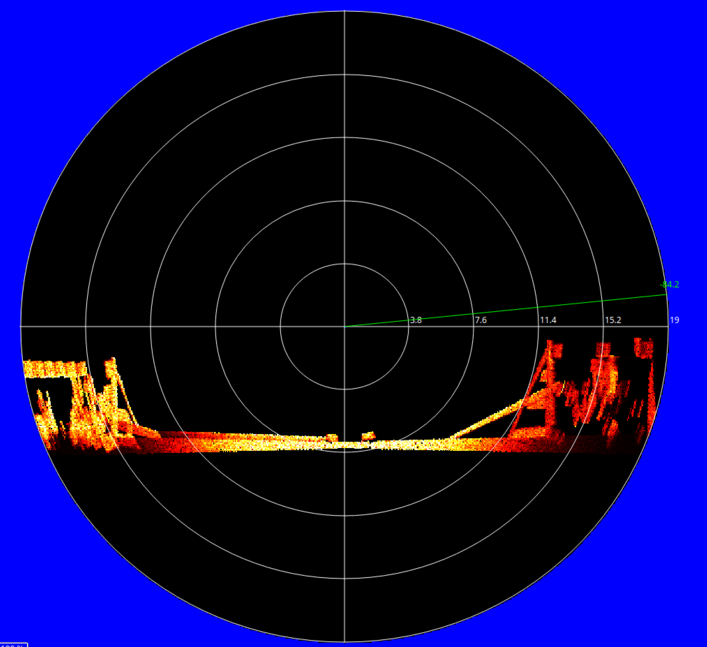
\includegraphics[width=0.4\paperwidth,height=6cm]{figs/msis_sim3}
        \label{fig:msis_sim3}
    }
    \captionsetup{justification=centering}
    \caption{Experiments using mechanical scanning imaging sonar in three
    different scenarios \subref{fig:msis_scene1}, \subref{fig:msis_scene2}
    and \subref{fig:msis_scene3}, and the respective processed simulated
    frames in horizontal axis in \subref{fig:msis_sim1} and
    \subref{fig:msis_sim2}, and vertical axis in \subref{fig:msis_sim3}.}
    \label{fig:msis}
\end{figure*}

The experimental scenarios provided enough variability of specific phenomena
usually found in real sonar images, such as acoustic shadows, noise
interference, surface irregularities and properties, distortion during
the acquisition process and gradient of acoustic intensities. However, our
sonar model also presented some limitations. For instance, the speckle noise
application is restricted to regions with acoustic intensity, as shown in
Figs. \ref{fig:fls_sim3} and \ref{fig:msis_sim1}. This fact is due to our
sonar model, defined in Eq. \ref{eq:2}, be multiplicative. In real sonar
images, the noise also granulates the shadows and blind regions. The sonar
simulator can be improved by inserting an additive noise to our model.
A second feature missing in simulated acoustic images are the ghost effects
caused by reverberation. This lacking part can be addressed by implementation
of a multi-path propagation model.

\subsection{Computational time}

Performance evaluation of the simulator was determined by considering the
suitability to run real-time applications. The experiments were performed
on a laptop with Ubuntu 16.04 64 bits, Intel Core i7 3540M processor
running at 3 GHz with 16GB DDR3 RAM memory and NVIDIA NVS 5200M video card.

The elapsed time of each sonar data is stored to compute the average time,
standard deviation and frame rate metrics, after $500$ iterations, as
summarized in Tables \ref{table:fls} and \ref{table:msis}. After changing
the device parameters, such as number of bins, number of beams and field
of view, the proposed approach generated the sonar frames with a high
frame rate, for both sonar types. Given the Tritech Gemini 720i, a real
forward-looking sonar sensor, with a field of view of $120^{\circ}$ by
$20^{\circ}$ and 256 beams, presents a maximum update rate of 15 frames
per second, the results allow the use of the sonar simulator for real-time
applications. Also, the MSIS data built by the simulator is able to
complete a $360^{\circ}$ scan sufficiently fast in comparison with a
real sonar as Tritech Micron DST. Moreover, for the FLS device, these
rates are superior to the rates lists by DeMarco \textit{et al}
\cite{demarco2015} ($330 ms$) and Saç \textit{et al} \cite{sac2015}
($2.5 min$). For MSIS type, to the best of our knowledge, there is no
previous work done for comparison.

According to previous results, since the number of bins is directly
proportional to sonar image resolution, as explained in Section
\ref{dev:sonardata}, this is also correlated with the computational time.
When the number of bins increases, the simulator will have a bigger scene
frame to compute, and generate the sonar data.

\begin{table*}[!h]
    \caption{Processing time to generate forward-looking sonar frames with different parameters.}
    \label{table:fls}
    \begin{center}
        \begin{tabular}{| c | c | c | c | c | c | c |}
            \hline
            \# of samples & \# of beams & \# of bins & Field of view & Average time ($ms$) & Std dev ($ms$) & Frame rate ($fps$) \\
            \hline
            500     & 128     & 500       & $120^{\circ}$ x $20^{\circ}$        & 54.7    & 3.7   & 18.3 \\ \hline
            500     & 128     & 1000      & $120^{\circ}$ x $20^{\circ}$        & 72.3	& 8.9   & 13.8 \\ \hline
            500     & 256     & 500       & $120^{\circ}$ x $20^{\circ}$        & 198.7	& 17.1  & 5.0  \\ \hline
            500     & 256     & 1000      & $120^{\circ}$ x $20^{\circ}$        & 218.2	& 11.9  & 4.6  \\ \hline
            500     & 128     & 500       & $90^{\circ}$ x $15^{\circ}$         & 77.4	& 11.8  & 12.9 \\ \hline
            500     & 128     & 1000      & $90^{\circ}$ x $15^{\circ}$         & 94.6	& 10.2  & 10.6 \\ \hline
            500     & 256     & 500       & $90^{\circ}$ x $15^{\circ}$         & 260.8	& 18.5  & 3.8  \\ \hline
            500     & 256     & 1000      & $90^{\circ}$ x $15^{\circ}$         & 268.7	& 16.7  & 3.7  \\ \hline
        \end{tabular}
    \end{center}
\end{table*}

\begin{table*}
    \caption{Processing time to generate mechanical scanning imaging sonar samples with different parameters.}
    \label{table:msis}
    \begin{center}
        \begin{tabular}{| c | c | c | c | c | c |}
            \hline
            \# of samples & \# of bins & Field of view & Average time ($ms$) & Std dev ($ms$) & Frame rate ($fps$) \\
            \hline
            500     & 500       & $3^{\circ}$ x $35^{\circ}$        & 8.8	    & 0.7  & 113.4 \\ \hline
            500     & 1000      & $3^{\circ}$ x $35^{\circ}$        & 34.5	& 1.6  & 29.0  \\ \hline
            500     & 500       & $2^{\circ}$ x $20^{\circ}$        & 10.3	& 0.6  & 96.7  \\ \hline
            500     & 1000      & $2^{\circ}$ x $20^{\circ}$        & 41.7	& 3.7  & 24.0  \\ \hline
        \end{tabular}
    \end{center}
\end{table*}

% ----------------------------------------------------------------------------------

\section{Conclusion and future work}
\label{conclusion}

A GPU-based approach for imaging sonar simulation is presented here.
The same model was able to reproduce the operation mode of two different
types of sonar devices (FLS and MSIS) over different scenarios. The real
sonar image singularities, such as multiplicative noise, surface
properties and acoustic shadows are addressed and represented in the
simulated frames. Specially for the shadows, the acoustic representation
can present information as useful as the insonified object. Considering
the qualitative results, the sonar simulator can be used by feature detection
algorithms, based on corners, lines and shapes. Also, the computation time
to build one sonar frame was calculated using different device settings.
The vertex and fragment processing during the underwater scene rendering
accelerates the sonar image building, and the metrics, such as the average
time, demonstrated that the performance is much close to real imaging
devices. These results allowed the use of this imaging sonar simulator
by real-time applications, such as obstacle detection and avoidance, and
object tracking. Finally, the reverberation effect is still missing on
our simulator to perform a more realistic sensing. The future inclusion
of this phenomena will probably change the reflected intensity model
and the computation time must be considered again. Next steps will
focus on expand the underwater acoustic characteristics, such as additive
noise and reverberation, and qualitative and computation\hyp{}efficiency
evaluations with other imaging sonar simulators.

% \nocite{*}
\bibliographystyle{model3-num-names}
\bibliography{elsarticle-template-3-num}

%% Authors are advised to submit their bibtex database files. They are
%% requested to list a bibtex style file in the manuscript if they do
%% not want to use model3-num-names.bst.

%% References without bibTeX database:

% \begin{thebibliography}{00}

%% \bibitem must have the following form:
%%   \bibitem{key}...
%%

% \bibitem{}

% \end{thebibliography}


\end{document}
